\documentclass[11pt,a4paper]{article}
\usepackage{ngerman}
\usepackage[ngerman]{babel}
\usepackage[utf8x]{inputenc}
\usepackage[T1]{fontenc}
\usepackage{lmodern}
\usepackage{marvosym}
\usepackage{amsfonts,amsmath,amssymb}
\usepackage{textcomp}
\usepackage{pifont}
\usepackage{ifpdf}
\usepackage[pdftex]{color}
\ifpdf
  \usepackage[pdftex]{graphicx}
\else
  \usepackage[dvips]{graphicx}\fi

\pagestyle{empty}

\usepackage[scale=0.775]{geometry}
\setlength{\parindent}{0pt}
\addtolength{\parskip}{6pt}

\def\firstname{Pascal}
\def\familyname{Bernhard}
\def\FileAuthor{\firstname~\familyname}
\def\FileTitle{\firstname~\familyname's Salz}
\def\FileSubject{Salz}
\def\FileKeyWords{\firstname~\familyname, Salz}

\renewcommand{\ttdefault}{pcr}
\hyphenation{ins-be-son-de-re}
\usepackage{url}
\urlstyle{tt}
\ifpdf
  \usepackage[pdftex,pdfborder=0,breaklinks,baseurl=http://,pdfpagemode=None,pdfstartview=XYZ,pdfstartpage=1]{hyperref}
  \hypersetup{
    pdfauthor   = \FileAuthor,%
    pdftitle    = \FileTitle,%
    pdfsubject  = \FileSubject,%
    pdfkeywords = \FileKeyWords,%
    pdfcreator  = \LaTeX,%
    pdfproducer = \LaTeX}
\else
  \usepackage[dvips]{hyperref}
\fi

\definecolor{firstnamecolor}{RGB}{56,115,179}
\definecolor{familynamecolor}{RGB}{56,115,179}
\hypersetup{pdfborder=0 0 0}

% Gleiche Schriftart für Hyperlinks
\urlstyle{same}


%  Gefrickel um URL-Links vernünftig umzubrechen
\makeatletter
\g@addto@macro\UrlBreaks{
  \do\a\do\b\do\c\do\d\do\e\do\f\do\g\do\h\do\i\do\j
  \do\k\do\l\do\m\do\n\do\o\do\p\do\q\do\r\do\s\do\t
  \do\u\do\v\do\w\do\x\do\y\do\z\do\&\do\1\do\2\do\3
  \do\4\do\5\do\6\do\7\do\8\do\9\do\0}
% \def\do@url@hyp{\do\-}

% Hiermit soll einer übervolle Box verhindert werden -- funktioniert sogar irgendwie
\g@addto@macro\UrlSpecials{\do\/{\mbox{\UrlFont/}\hskip 0pt plus 1pt}}
\makeatother

% Farben werden hier definiert
\definecolor{MidnightBlue}{RGB}{0,103,149}


\begin{document}
\sffamily   % for use with a résumé using sans serif fonts;
%\rmfamily  % for use with a résumé using serif fonts;
\hfill%
\begin{minipage}[t]{.6\textwidth}
\raggedleft%
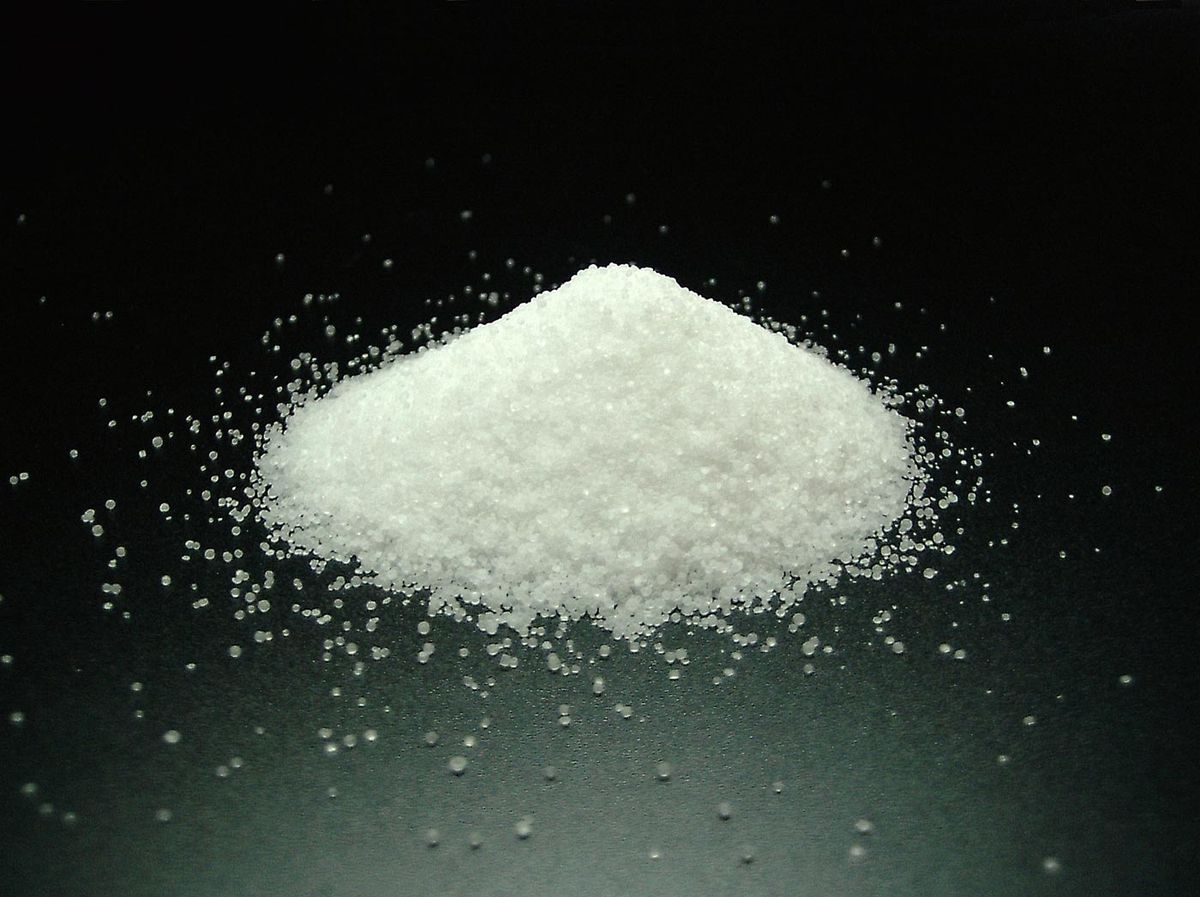
\includegraphics[width=0.55\textwidth]{Speisesalz.jpg}


\end{minipage}\\[0.5em]
%
{\color{firstnamecolor}\rule{\textwidth}{.25ex}}
%
\begin{minipage}[t]{.4\textwidth}
	\raggedright%
	% {\bfseries {\color{firstnamecolor}
	\vspace*{1em}
%	\textbf{Geschichte der Habsburger -- Flaggen} \\
%	 \\[.35ex]
	% }}
	\small%
%	Wolframstraße 89-92\\
%	12105 Berlin
\end{minipage}
%
\hfill
%
\begin{minipage}[t]{.4\textwidth}
	\raggedleft % US style
	\today
	%April 6, 2006 % US informal style
	%05/04/2006 % UK formal style
\end{minipage}\\[2.2em]


{\bfseries \color{familynamecolor}{{\LARGE Die Geschichte des Salzes}}}\\[0.75em]

\section*{\textsf{Die Bedeutung von Salz für die Menschen}}

\begin{itemize}
\item Salz (Natriumchlorid) ist für den menschlichen Körper unverzichtbar und somit ein wichtiger Bestandteil der Ernährung\\
\ding{225} Salz sorgt für die Regulierung des Wasser im Körper und ist für Muskeln und Knochen von Bedeutung

\item lange Zeit war Salz neben Alkohol und Räuchern eines der wenigen Mittel, Lebensmittel haltbar zu machen

\item bis zum 19. Jahrhundert war der Bedarf an Salz größer, als die verfügbare Menge\\
\ding{225} Salz war so wertvoll, dass es auch als das '\textsl{weiße Gold}' bezeichnet wurde


\end{itemize}




\subsection*{\textsf{Salzhandel in der Antike}}

\begin{itemize}

\item bereits die Babylonier und Ägypter nutzten Salz zur Konservierung

\item seit der Steinzeit wird in Europa Salz in Bergwerken abgebaut, das älteste bekannte Salzbergwerk ist über 3000 Jahre alt und befindet sich in Hallstatt (Oberösterreich)\\
\ding{225} die Hallstättische Steinzeitkultur ist nach dem Ort der Salzgewinnung benannt

\item die Phönizier waren in der Antike (1200-900 vor Christus) die ersten, die Salz in großem Maßstab handelten\\
\ding{225} die lieferten Salz und Wein aus dem Mittelmeergebiet nach Nordeuropa und tauschten diese gegen Pelze, Bernstein und Zinn ein

\item die Kelten begann um 1000 v.Chr. mit dem Abbau von Salz in Bergwerken\\
\ding{225} \textsl{Hall} war das keltische Wort für Salz (Bad Reichenhall, Hallstatt, Halle, etc.)

\item im Mittelmeerraum wurde Salz in Meergärten durch Verdunstung von Meerwasser gewonnen

\item im Römischen Reich existierte ein 'Salzverteilernetz' aus spezialisierten Kaufleuten, den \textsl{salarii}, die Salz bis in die entlegendsten Regionen des Reiches transportierten\\
\ding{225} dieses Salznetz funktionierte so reibungslos, dass der Preis für das Gut im Vergleich zum Mittelalter sehr stabil war


\item diese Preisstabilität und die geregelte Versorgung ermöglichte es den Römern, Salz als Zahlungsmittel zu verwenden\\
\ding{225} die römischen Legionäre erhielten ihr Gehalt im Form von Salz, das sog. \textsl{salarium} (salary, salaire, Salär)


\item der Verkauf von Salz (wie auch von Waffen und Getreide) an die Feinde des Römischen Reiches war streng verboten


\end{itemize}



\subsection*{\textsf{Salz im Mittelalter Europas}}

\begin{itemize}

\item mit dem Niedergang und Ende des Römischen Reiches kam der europäische Salzhandel zum Erliegen\\
\ding{225} Salz musste lokal gewonnen werden, z.B. in sogenannten \textsl{Solen}

	\begin{itemize}
	\item in Solen wird mit Salz gesättigtes Wasser durch Verheizen von Brennholz verdampft, das Salz bleibt zurück
	\item der große Bedarf an Brennholz hat zum Entstehen der Heidelandschaft um Lüneburg beigetragen\\
	\ding{225} keine nachhaltige Form der Salzgewinnung
	\end{itemize}

\item Salzhandel über lange Distanzen war im mittelalterlichen Europa nicht mehr möglich, so dass nicht mehr das günstigere Meersalz aus der Mittelmeerregion verwendet wurde\\
\ding{225} die Salzbergwerke im Alpenraum erlebten einen Wiederaufschwung

\end{itemize}


\subsection*{\textsf{Kaisertum Österreich}}

\begin{itemize}

\item vor der Schlacht von Austerlitz hatte der damalige König Östereichs Franz II sich zum Kaiser Franz I ausgerufen, um Ranggleichheit mit Napoleon und dem russischen Zaren zu haben\\
\ding{225} \textsl{Drei-Kaiser Schlacht}

\item nach Druck des ungarischen Adels wurde das Kaisertum Österreich in die Österreichisch-Ungarische Monarchie umgewandelt\\
\ding{225} der österreichische Kaiser war zugleich König Ungarns\\
\ding{225} K.u.K Monarchie -- Kaiser und König Monarchie

\item am 11. November 1918 verzichtet Kaiser Karl I auf alle Staatsgeschäfte\\
\ding{225} keine formale Abdankung\\
\ding{225} kaiserliche Familie floh 1919 in die Schweiz, um einer Verhaftung zu entgehen


\end{itemize}

\section*{\textsf{Flaggen der Österreichs, Deutschlands und der Schweiz}}


\subsection*{\textsf{Schweizer Flagge}}

\begin{itemize}

\item die Schweizer Flagge geht auf die Zeit der Eidgenössischen Kriege zurück

\item jeder Kanton führte im Krieg seine eigene Fahne mit sich, eine Schweizer Fahne gab es in der damaligen Zeit noch nicht

\item die Soldaten des Kantons Schwyz hatten eine rote Flagge und durften seit ihrer Unterstützung Rudolfs IV von Habsburg im Krieg gegen Burgund das weiße Kreuz als Symbol der Kreuzigung Christi hinzufügen

\item je größer die Eidgenossenschaft wurde, desto schwieriger wurde es, die Soldaten der vielzähligen Kantone voneinander zu unterscheiden\\
\ding{225} das weiße Kreuz wurde zum gemeinsamen Erkennungszeichen

\item das Schweizer Kreuz mit seinen gleichen Seitenverhältnissen war zugleich eine Abgrenzung der Schweizer Söldner gegen das Andreaskreuz der deutschen Landsknechte


\end{itemize}



\subsection*{\textsf{Flagge Österreichs}}

\begin{itemize}

\item die Farben Rot-Weiß-Rot der österreichischen Fahne geht auf das Schild des Adelsgeschlechts der Babenberger zurück

\item nachdem die Habsburger 1270 mit den Besitzungen der Babenberger belehnt wurden, integrierten sie dessen Farben in das eigene Wappen

\item ab dem 15. Jahrhundert wurde Rot-Weiß-Rot endgültig zum Wappen Österreichs


\end{itemize}



\subsection*{\textsf{Deutsche Flagge}}


\begin{itemize}

\item Vorläufer der Kombination Schwarz-Rot-Gold war das Reichsbanner der Heiligen Römischen Reiches Deutscher Nation (Schwarzer Adler mit roten Krallen auf goldenem Grund)

\item die moderne deutsche Fahne aus Schwarz-Rot-Gold hat seinen Ursprung in den Befreiungskriegen 1813 gegen Napoleon\\
\ding{225} die Freiwilligen des Lützowschen Freikorps setzte sich vor allem aus Studenten mit unterschiedlichster Kleidung zusammen\\
\ding{225} alle Bekleidung wurde schwarz gefärbt und goldene Messingknöpfe sowie rote Kragen und Aufschläge aufgenäht\\
\ding{225} aus diesem Freikorps gründete sich die 'Urburschenschaft', die Schwarz-Rot-Gold zu ihrer Fahne wählten\\
\ding{225} Wahlspruch: \textsl{Aus der Schwärze (schwarz) der Knechtschaft durch blutige (rot) Schlachten ans goldene (gold) Licht der Freiheit}

\item am vierten Jahrestag der Völkerschlacht von Leipzig zog die Urburschenschaft unter der 'Deutschen Flagge' und der Losung 'Nur im Ganzen heil' auf die Wartburg

\item die Farben Schwarz-Rot-Gold wurden zur Zeit des Deutschen Bundes (1815-1866) zu den deutschen Nationalfarben

\item die Revolutionäre, welche die Einheit Deutschlands als Republik und nichts als Monarchie forderten, nahmen die dreifarbige Fahne in Anlehnung an die französische Trikolore

\item nach Ende des Kaiserreiches wurde von der Weimarer Republik Schwarz-Rot-Gold als nationales Flagge gewählt


\end{itemize}



\end{document}